\documentclass[a4paper, oneside]{article}
\usepackage[T1]{fontenc}
\usepackage[utf8]{inputenc}
\usepackage[english]{babel}
\usepackage{frontespizio}
\usepackage{graphicx}
\usepackage{listings}
\usepackage{scrextend}
\usepackage[margin=1.2in]{geometry}
\usepackage[font=small,labelfont=bf]{caption}
\usepackage{url}
\usepackage{verbatim}

\begin{document}
\selectlanguage{english}
\baselineskip 13pt

% ---- FRONTESPIZIO ----- 
\begin{frontespizio} 
\Preambolo{\renewcommand{\frontpretitlefont}{\fontsize{15}{12}\scshape}}
\Istituzione {University of Pisa}
\Divisione {Scuola di Ingegneria}
\Corso [Laurea]{Artificial Intelligence and Data Engineering}
\Annoaccademico {2019--2020}
\Titolo {Task2 documentation}
\Filigrana [height=4cm,before=0.28,after=1]{./images/stemma_unipi.png}
\Rientro {1cm}
\Candidato {Giacomo Mantovani}
\Candidato {Stefano Poleggi}
\Relatore {Prof. Pietro Ducange}
 \Punteggiatura {}
\end{frontespizio}

\clearpage

% ----- INDICE -----
	\tableofcontents\thispagestyle{empty}
	\clearpage


\section{Introduction}\pagenumbering{arabic}
The \textbf{TweetQuake} application offers a real-time earthquake detection service in Italy. When the application opens up it will start fetching tweets and analyzing them to recognize ones related to an earthquake.
The application will show the number of tweets analyzed so far and the corresponding number of earthquake tweets and non-earthquake tweets. When some earthquake tweets are recognized the application show a warning message, if there is a trend of earthquake tweets then the application will show an emergency message.
\vspace{5mm}
\begin{figure}[h]
\centering
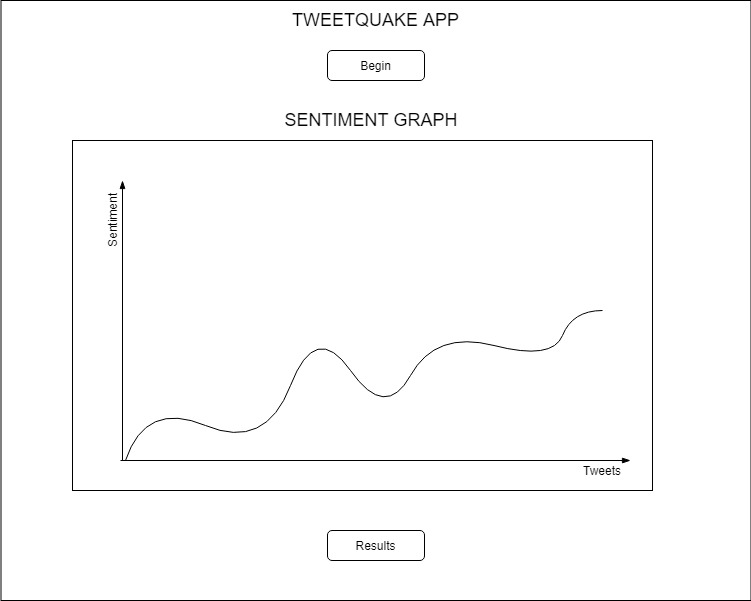
\includegraphics[width=\textwidth]{./images/diagrams/HomeMockup} 
\caption{Home Page Mockup}
\label{fig:mockup}
\end{figure}

\begin{figure}[h]
\centering
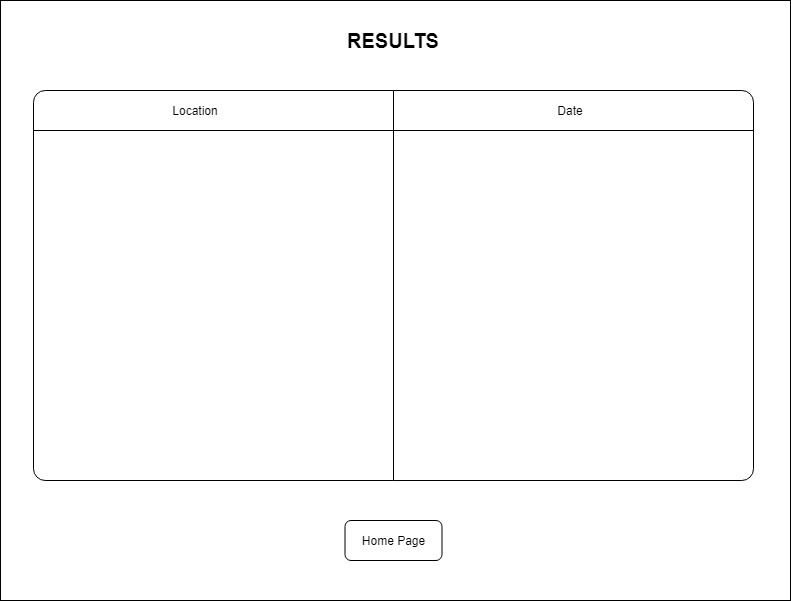
\includegraphics[width=\textwidth]{./images/diagrams/Charts} 
\caption{Results Page Mockup}
\label{fig:mockup}
\end{figure}

\clearpage

\section{Analysis and workflow}

% ----- REQUIREMENTS -----
\subsection{Requirements}

\subsubsection{Functional requirement}
The system has to iteratively perform the following operations: 
\begin{itemize}
\item Real-time fetching of tweets.
\item Perform a classification of the tweets and obtain the label (earthquake or non-earthquake).
\item When an earthquake tweet is regocnized send a warning message.
\item When an earthquake tweet trend is recognized send an emergency message.
\end{itemize}
\vspace{2mm}

\subsubsection{Non-functional requirements}
\begin{itemize}
\item Usability, ease of use and intuitiveness of the application by the user.
\item The system should provide a high level of accuracy.
\end{itemize}

\clearpage

% ----- USE CASES -----
\subsection{Use Cases}

\textbf{Actors}
\begin{itemize}
\item{User: this actor represents a user of the application}
\item{System: this actor represent the system}
\item{Twitter: this actor represent the Twitter service}
\end{itemize}

\subsubsection{Use Cases Description}
\begin{itemize}
\item Twitt Search : This use case can be performed by the user to start the real-time tweet fetching.
\item Retrive Tweet: This use case represents the action of getting a tweet from twitter.
\item Twitter Connection: This use case represents the connection with the Twitter service.
\item HTTP Request for Connection: This use case represents the Request for the connection to Twitter Service.
\item HTTP Response for Connection: This use case represents the Response for the connection to Twitter Service.
\item HTTP Request for Tweets: This use case represents the Request for tweets.
\item HTTP Response for tweets: This use case represents the Response for tweets.
\item Perform Text Analysis: This use case represents the process of Text analysis performed by the system ( for more informations check paragraph < add paragraph num > )
\item Apply Classification Algorithm: This use case represents the classification of the tweets performed with the classifier generated by the "Generate Classifier" use case.
\item Show Warning/Emergency Message: This use case displays an error message if some earthquake tweet are recognized.
\item Display Results: This use case shows the results of the classification.
\item Generate Classifier: This use case is performed automatically by the system and it generates a classifier using a training set. 
\item Browse Tweets: The system browses the data on the database.
\item Train the classifier: Perform an algorithm to generate the classifier.
\item Stop Real-Time fetching: This use case allows the user to stop the real-time tweets fetching.
\end{itemize}

\begin{minipage}{\linewidth}
\begin{center}
\vspace{8mm}
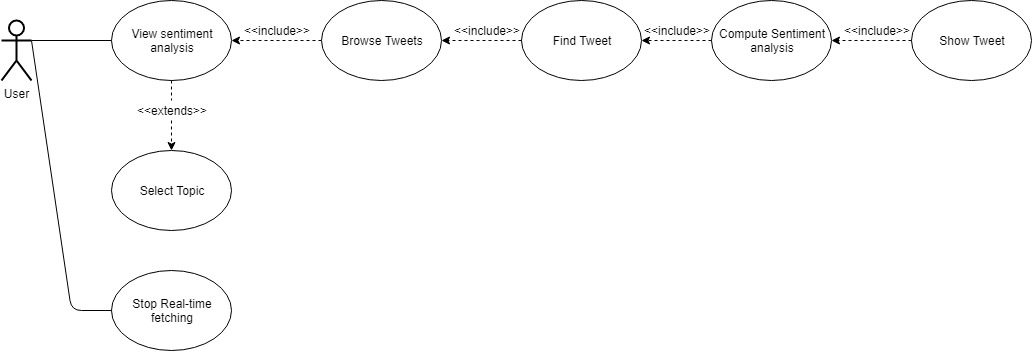
\includegraphics[ width=0.55\textheight]{./images/diagrams/UseCase} 
\captionof{figure}{Use cases diagram}
\vspace{3mm}
\end{center}
\end{minipage}


\clearpage
\subsection{System Flow Diagram}
\begin{minipage}{\linewidth}
\begin{center}
\vspace{8mm}
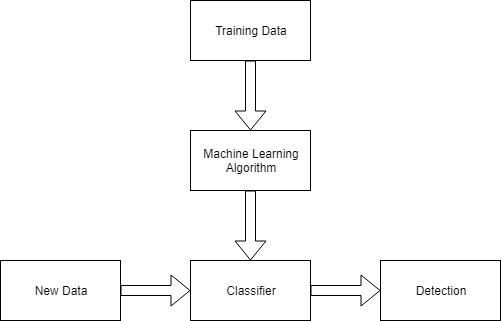
\includegraphics[ width=0.6\textheight]{./images/diagrams/Flow Diagram} 
\captionof{figure}{Flow Diagram}
\vspace{3mm}
\end{center}
\end{minipage}

\clearpage
\subsection{System Architecture}
\begin{minipage}{\linewidth}
\begin{center}
\vspace{8mm}
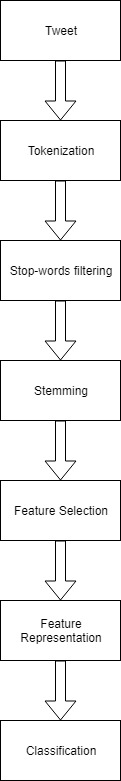
\includegraphics[ width=0.13\textheight]{./images/diagrams/Process} 
\captionof{figure}{Text Analysis Process}
\vspace{3mm}
\end{center}
\end{minipage}


\clearpage
\subsection{Analysis of entities}
This diagram represents the main entities of the application and the relations between them.
\begin{minipage}{\linewidth}
\begin{center}
\vspace{4mm}
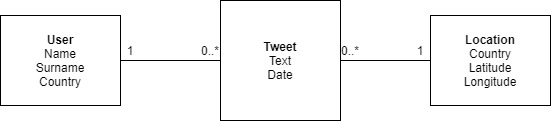
\includegraphics[width = 0.2\textwidth]{./images/diagrams/Uml Analysis diagram} 
\vspace{2mm}
\captionof{figure}{UML analysis diagram}
\label{fig:useCases}
\end{center}
\end{minipage}



\clearpage
% ----- DESIGN -----
\section{Design}

\subsection{Database Choice}
After the analysis phase, which has been carried out so far, we start with the design of the \textbf{TweetQuake} application. We decide to use MongoDB as data support. Its document-based structure is very useful for the large amount of data that we need to maintain and access, as well as its high scalability, qualities that we do not find in a relational database.
\subsection{Software architecture}
The application is designed over 3 different layers, see figure \ref{fig:architecture_diagram}:
\begin{itemize}
\item Front-end
\item Middleware
\item Back-end
\end{itemize}
\vspace{5mm}
\begin{minipage}{\linewidth}
\begin{center}
\vspace{1mm}
\includegraphics[height = 100mm]{./images/diagrams/architecture} 
\vspace{6mm}
\captionof{figure}{Software architecture diagram\\}
\label{fig:architecture_diagram}
\end{center}
\end{minipage}
\vspace{7mm}
\clearpage


\subsection{Populating the database}
The dataset used in the \textbf{TweetQuake} application was created by scraping Tweets, using Twitter4j which is a java library for the Twitter API. Given location and tags to search for, this API returns the informations about the tweets matching those parameters. To build the Database two different queries have been used: 
\begin{itemize}
\item The first query selects the tweets in Italy matching the tags {\#}terremoto, {\#}magnitudo and {\#}earthquake.
\item The second query selects the tweets in Italy without tags.
\end{itemize} 
After that the text of the tweets have been stored in the database and the labels have been added manually to obtain a good training (and test) set to generate a classifier.
The second query is necessary to obtain better results because without the tweets obtained from it the classifier would suffer from overfitting.\\

<code here>

\clearpage

% ----- IMPLEMENTATION -----
\section{Implementation}
\subsection{Used technologies}
The application is developed in java programming language, version 11.0.4, and in JavaFX system to create the GUI, version 11, so it should run on each platform in which JVM is installed, but the application is tested and guardantee on Ubuntu 16 and Window OS. Moreover Maven is used  to build and mantain the project, version 3.8.0. \\
The java driver for mongo manage the comunication between client application layer and mongo backend layer, version 3.11.2.\\ 
For the backend layer it is used MongoDB, version 4.2.\\
So this application is tested using these technologies, considering these particular versions: for other versions the correct execution isn't guaranteed .\\

\subsubsection{Declaration of class Tweet}
The following java-code shows a declaration of the class Tweet.
\vspace{2mm}
\\ <code here>
\vspace{5mm}

Another foundamental class is SQLManager, that manages the db-connection and the related operations.

\subsection{Create}
Adding a tweet to the database.
\vspace{2mm}
 \\<Code here>
\vspace{5mm}

\subsection{Read}
This functionality returns a list of tweets.
\vspace{2mm}
\\<code here>
\vspace{5mm}

\clearpage

\subsection{Text Analysis}
This functionality performs a text analysis of a tweet.
\vspace{2mm}
\\<code here>
\vspace{5mm}

\clearpage

\subsection{GUI}
There is an fxml documents which describes the objects showed in the GUI interface of the  page.
\begin{itemize}
\item Home.fxml
\end{itemize}
In addiction there is a class, called Controller, that is in charge of handling events of the objects defined in the associated fxml document.
\begin{itemize}
\item HomeController.java
\end{itemize}

\clearpage
% MANUAL%
\section{User Manual}
When you first run the application, the interface you get is the login one, figure~\ref{fig:screen0}. \\

<login page image--> image name: screen0>\\

In case you are not registered you can click the link at the bottom of the page to be redirected to a register page, figure~\ref{fig:screen1}, otherwise you can sign in the application and by default you get the interface shown in figure~\ref{fig:screen2}\\

<register page image --> image name: screen1>\\

<Application home page after login --> image name: screen2> \\

From here you can search for a film by typing in the relative field and clicking the search button. You'll get a list of films that contains the text entered in the table below. Now you can select a film from the table and all the informations will be shown in the right pane of the application, figure~\ref{fig:screen3}. In the bottom right you are able to add a vote from 1 to 10 for the selected film.\\

<homepage after searching a film and selectiong one --> image name: screen3>\\

In the top left of the page there are two tabs. by default after the login you are in the Home tab, by clicking the Analytics Tab you will see the following page.

<analytics tab page --> image name: screen4>\\

Here you have a choice box (left) to select what kind of analytics you want to be performed from the existing ones, and another one to apply a filter (right), figure~\ref{fig:screen5}. \\

<default analytics page --> image name: screen5>\\

After selecting an analytics you will see the results in the table below, and for some of them you will get a piechart aswell, figure~\ref{fig:screen6}\\

<analytics page after performing analytics -->image name: screen6>\\

To log out, just click on the appropriate button at the bottom.


\end{document}
